%----------------------------------------------------------------------------------------
%	PACKAGES AND OTHER DOCUMENT CONFIGURATIONS
%----------------------------------------------------------------------------------------


\documentclass[12pt,oneside,final,a4paper]{report}
\usepackage{generators/imports}
%\makeglossaries      % alt 1
\makenoidxglossaries  % alt 2

\renewcommand*{\acronymname}{List of Acronyms and Abbreviations}
\renewcommand{\glsnamefont}[1]{\textbf{#1}}

%Create acronyms here.
%\newacronym{nn}{NN}{Neural Network}
\newacronym{gnn}{GNN}{Graph Neural Network}
\newacronym{vcs}{VCS}{Version Control System}
%\newacronym{ml}{ML}{Machine Learning}
%\newacronym{ai}{AI}{Artificial Intelligence}
\newacronym{co}{CO}{Combinatorial Optimization}
\newacronym{mwm}{MWM}{Maximum Weighted Matching}
\newacronym{mis}{MIS}{Maximal Indepndent Set}


%You can also do explanations.
\newglossaryentry{git}{name={Git},
    description={Git and GitHub is a \gls{vcs} for tracking changes in computer files and coordinating work on those files among multiple people}}
\newglossaryentry{ga}{name={Greedy Algorithm},
    description={Algorithm that usually tries to sort input based on some criteria and then naively produces the answer based on the order of sorting}}
\newglossaryentry{ai}{name={Artificial Intelligence},
    description={Artificial Intelligence is a field of study regarding intelligence simulated by computers. Where intelligence is meant in context of human intelligence}}
\newglossaryentry{ml}{name={Machine Learning},
    description={Machine Learning studies algorithms that learn general patterns and make predictions based on some form of input. It is one form of \gls{ai}}}
\newglossaryentry{nn}{name={Neural Network},
    description={Neural Network is one of many technologies used in\gls{ml}}}


\begin{document}
\begin{titlepage}

\newcommand{\HRule}{\rule{\linewidth}{0.5mm}} % Defines a new command for the horizontal lines, change thickness here

\center % Center everything on the page
 
%----------------------------------------------------------------------------------------
%	HEADING SECTIONS
%----------------------------------------------------------------------------------------

\textsc{\LARGE University of Bergen \\ Department of Informatics}\\[1.5cm] % Name of your university/college

%----------------------------------------------------------------------------------------
%	TITLE SECTION
%----------------------------------------------------------------------------------------

\HRule \\[0.5cm]
\begin{Huge}
	\bfseries{Solving Maximum Weighted Matching problem using Graph Neural Networks}\\[0.7cm] % Title of your document
\end{Huge}
\HRule \\[0.5cm]

%----------------------------------------------------------------------------------------
%	AUTHOR SECTION
%----------------------------------------------------------------------------------------

\large \emph{Author:} Nikita Zaicev\\
\large \emph{Supervisor:} Fredrik Manne\\[2cm]

%----------------------------------------------------------------------------------------
%   LOGO SECTION
% 	This will require the graphicx package
%	Change the line to comment if you only want the UiB Logo
%	Logo for other faculties here: http://kapd.h.uib.no/profilmanual/99LastNed/99a_lastned.html
%----------------------------------------------------------------------------------------

\centerline{
\includegraphics[scale=1.9]{figures/canvasWithFaculty}}
%\centerline{
\includegraphics[scale=0.15]{figures/canvas}}  %change for your faculty

%----------------------------------------------------------------------------------------
%	DATE SECTION
%----------------------------------------------------------------------------------------

{\large \monthyeardate\today}\\[3cm] % Date, change the \today to a set date if you want to be precise

%----------------------------------------------------------------------------------------
%	LOGO SECTION
%----------------------------------------------------------------------------------------

\vfill % Fill the rest of the page with whitespace

\end{titlepage}
 % This is the titlepage
\pagenumbering{roman}

\begin{abstract} 

\noindent In this work we tried to train a \gls{gnn} to solve the Maximum Weighted Matching problem on graphs. 

\end{abstract}

\renewcommand{\abstractname}{Acknowledgements}
\begin{abstract}
	I want to thank Fredrikk Manne, Kenneth Langedal and Johannes Langguth for helping me with this work.
	
	\vspace{1cm}
	\hspace*{\fill}\texttt{Nikita Zaicev}\\ 
	\hspace*{\fill}\today
\end{abstract}
\setcounter{page}{1}
\newpage
{
\tableofcontents 
\let\cleardoublepage\clearpage \listoffigures 
\let\cleardoublepage\clearpage \listoftables 
\let\cleardoublepage\clearpage \lstlistoflistings
}
\pagenumbering{arabic}
\setcounter{page}{1}
\setlength{\parskip}{0.5cm plus4mm minus3mm}  

\chapter{Introduction}

This chapter is dedicated to the general introduction of the problem at hand and previous work and research that is relevant for this project.

\gls{ml} and Neural Networks have shown to be extremely potent and versatile in solving vast variety of problems across different fields. One research field that has been popular and challenging in the last few years is \gls{co}. \gls{co} includes problems such as \gls{mis} and \gls{mwm}. Such problems can be viewed in the context of graphs. \gls{gnn} is a subclass of Neural Networks designed specifically for solving problems related to graphs, but there are many problems that have not yet been solved efficiently with \gls{gnn}s. This work attemps to find out whether a \gls{gnn} can be worth using for solving \gls{mwm} 

\section{Background}

Many researches have been done related to \gls{gnn}s in the past years and some of them have shown mixed results. Lorenzo Brusca and Lars C. P. M. Quaedvlieg et al. \cite{brusca2023maximum} showed a self-training \gls{gnn} for \gls{mis}

\section{Project structure}

The rest of this document has the following structure:

\begin{enumerate}
\item Approach
\item Training
\item Results
\item Conclusion
\end{enumerate}


\subsection{Listings}
You can do listings, like in Listing~\ref{ListingReference}
\begin{lstlisting}[caption={[Short caption]Look at this cool listing. Find the rest in Appendix~\ref{Listing}},label=ListingReference]
$ java -jar myAwesomeCode.jar
\end{lstlisting}

You can also do language highlighting for instance with Golang:
And in line~\ref{LineThatDoesSomething} of Listing~\ref{ListingGolang} you can see that we can ref to lines in listings.

\begin{lstlisting}[caption={Hello world in Golang},label=ListingGolang,escapechar=|]
package main

import "fmt"

func main() {
    fmt.Println("hello world") |\label{LineThatDoesSomething}|
}

\end{lstlisting}

\subsection{Figures}

Example of a centred figure
\begin{figure}[H]
    \centering
    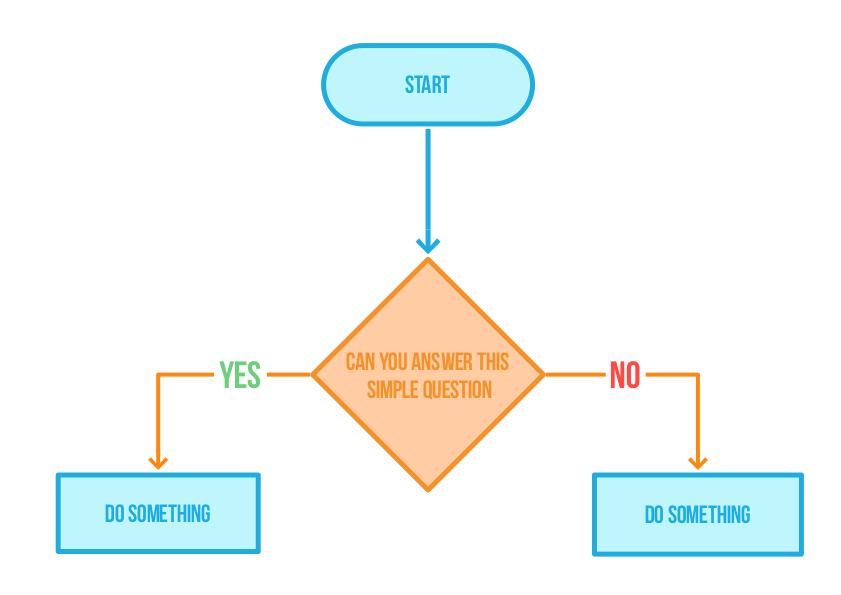
\includegraphics[scale=0.5]{figures/Flowchart}
    \caption{Caption for flowchart}
  	\medskip 
	\hspace*{15pt}\hbox{\scriptsize Credit: Acme company makes everything \url{https://acme.com/}}
    \label{FlowchartFigure}
\end{figure}

\subsection{Tables}

We can also do tables. Protip: use \url{https://www.tablesgenerator.com/} for generating tables.
\begin{table}[H]
\centering
\caption{Caption of table}
\label{TableLabel}
\begin{tabular}{|l|l|l|}
\hline
Title1 & Title2 & Title3 \\ \hline
data1  & data2  & data3  \\ \hline
\end{tabular}
\end{table}

\subsection{\gls{git}}

\gls{git} is fun, use it!

% Include more chapters as required.
%%=========================================

% Alternative 1 of printing glossaries & acronymes
%\renewcommand{\glossarypreamble}{\footnotesize}
%\printglossary[style=super, type=\glsdefaulttype] \let\cleardoublepage\clearpage
%\printglossary[style=super, type=\acronymtype]


%Alternative 2
%Simplified way of printing glossaries, slower than alt 1, but has better compatibility
\printnoidxglossaries

% Include more appendices as required.
%%=========================================
\clearpage
\DeclareRobustCommand{\VAN}[3]{#3}
\addcontentsline{toc}{chapter}{Bibliography}
\bibliographystyle{generators/myplainnat}
\bibliography{generators/refs}
\appendix
\titleformat{\chapter}[display]
  {\normalfont\large\bfseries}% <- font for label "Appendix A", default \huge
  {\chaptertitlename\ \thechapter}
  {20pt}
  {\large}% <- font for title, default \Huge

\chapter{Generated code from Protocol buffers}

\begin{lstlisting}[caption={Source code of something},label=Listing]
System.out.println("Hello Mars");
\end{lstlisting}
\end{document}
